\chapter{Introduction}
\label{chapter:intro}

%iad_field
In our modern times when we strive to automate every menial task that was resolved by human labor, one of the fields that have been the most important is the industrial manufacturing processes. In improving the process of production, the key point is to ensure the reliability of the process and the quality of the produce. Throughout the recent years, the use of Machine Learning algorithms, specifically Computer Vision models, have showed to be a powerful tool in detecting the defects(called anomalies in the field of machine learning). Therefore, a new field: Industrial Anomaly Detection was formed, which focuses on researching and developing efficient computer vision models in the field. There are generally two types of architectures in the industrial anomaly detection models: feature embedding based architectures and reconstruction based architectures. Most contemporary models are trained without supervision and they, due to the lack of large scale image dataset of industrial objects and the unbalanced nature of available datasets towards nominal samples, rely on the feature space of a pre-trained model.

%iad_arch
The training process depends on the architecture of the model. In feature-embedding types of architectures, usually the training process involves performing a feature extractions and saving them with various modifications. Thereafter, during inference same feature extraction applied to the image being inferred followed by various statistical methods used to calculate the anomaly score of the sample. An example for the feature embedding architecture can be a model PatchCore, which saves nominal features in the memory bank after applying neighborhood aggregation and utilized k-nearest neighbor method to calculate an anomaly score. In reconstruction based methods, autoencoder models is trained either on the features extracted by the pre-trained model or the pre-trained model is used as an encoder inside the autoencoder. For example, in the RealNet model multiple autoencoders are trained on the layers of the feature extractor model. 

\begin{figure}[t]
\begin{center}
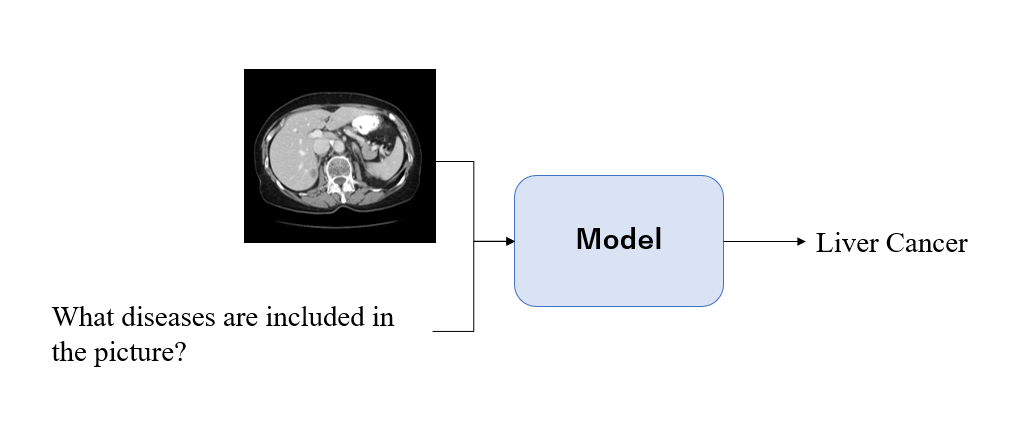
\includegraphics[width=1.0\linewidth]{Chapter_1/chap1_medvqa.png}
\end{center}
   \caption{Medical Visual Question Answering (VQA) \cite{liu2021slake} is a task where the model receives medical images and corresponding questions as input and produces accurate answers as the output.
}
\label{fig:medvqa}
\end{figure}

\begin{figure}[t]
\begin{center}
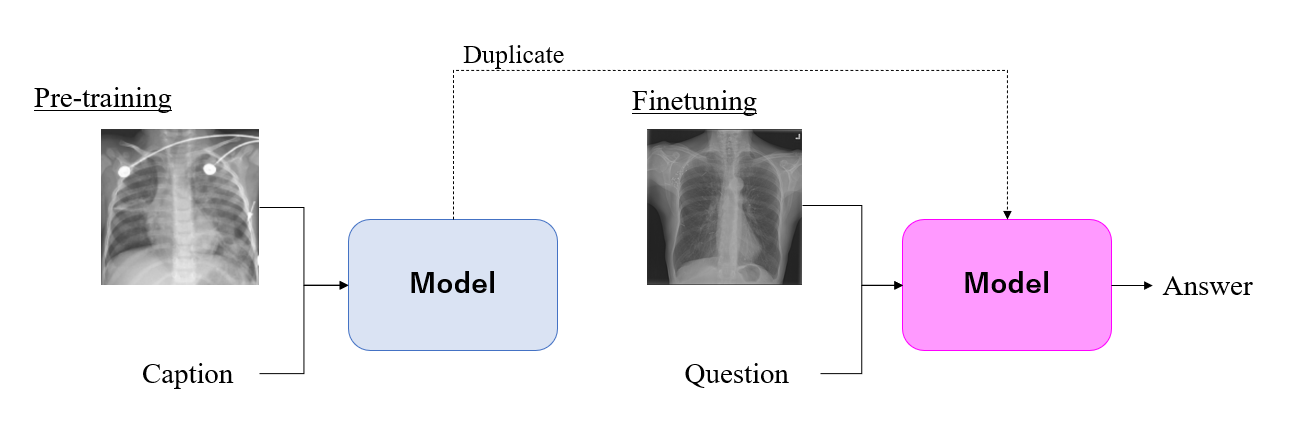
\includegraphics[width=1.0\linewidth]{Chapter_1/chap1_pretrain_finetune.png}
\end{center}
   \caption{Pre-training followed by finetuning: The approach involves pre-training the model on a large-scale medical image-caption dataset \cite{Pelka2018RadiologyOI}, and subsequently finetuning it specifically for the task of medical visual question answering \cite{liu2021slake}.
}
\label{fig:pretrainFinetune}
\end{figure}

\begin{figure}[t]
\begin{center}
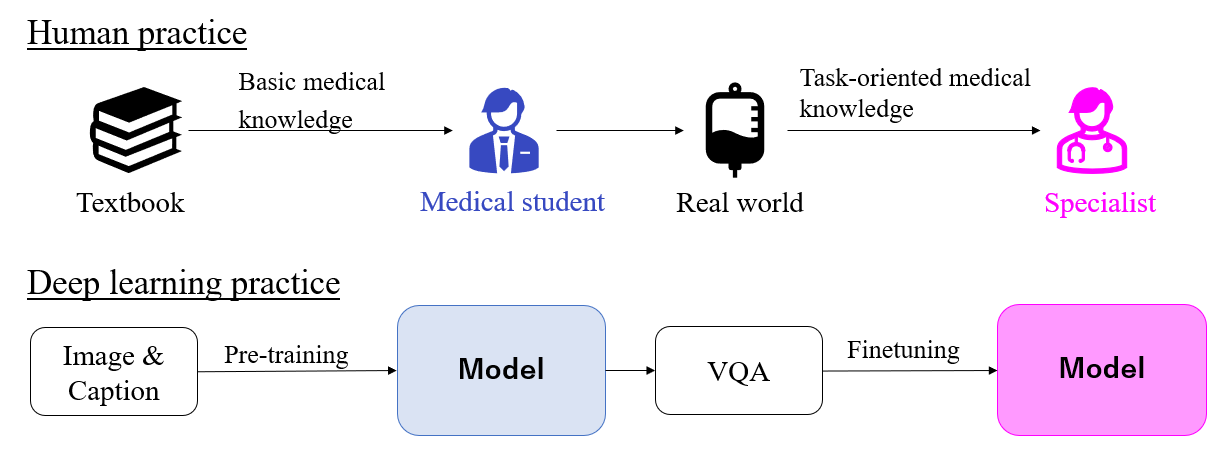
\includegraphics[width=1.0\linewidth]{Chapter_1/chap1_medstudent.png}
\end{center}
   \caption{Comparing model learning to medical student training
}
\label{fig:medstudent}
\end{figure}

In this paper we hypothesize that using ImageNet pre-trained models as feature extractors in industrial anomaly detection models can be a potential bottleneck of performance due to the generalized nature of the ImageNet dataset. There is a large representation mismatch between ImageNet which contains a large quantity of natural samples whereas the IAD requires features which represent industrial objects more accurately. Our hypothesis implies that most if not all existing models could benefit from a more specialized feature space which is extracted from datasets with focus on more industrial settings rather than being general or having natural samples.

In order to address this issue the thesis proposes to generate a feature space that would represent the type of data that is used in industrial anomaly detection tasks. In order to accomplish this task, we propose extracting an industrial setting sub-datasets from a large multi-purpose dataset, followed by performing a training on the extracted dataset to have a feature extractor. Throughout this process it is important to choose appropriate dataset to extract from, a proper self supervised learning method and an accurate extraction method. All three parts of the pipeline are important and have to be a deliberate choice, however the most important part and the defining factor for the quality of the extracted features is the extraction method.

In this thesis we opted to utilize a ResNet50 model trained on the dataset curated by hand. However, in this thesis, we will also be discussing other possible options for industrial image extractors. Due to the unlabeled nature of the extracted dataset by the method of our choice, this work will use the DINO unsupervised learning method on all experiments as a feature learning tool. The choice is also motivated by the capability of DINO to train both Vision Transformer and Convolution based networks.

To evaluate the accuracy of different feature spaces against each other, we use PatchCore as the main industrial anomaly detection model. All pre-trained models are to be used as backbones for the model and evaluated on the accuracy of the model on MVTechAD dataset. Firstly, we perform experiments on ViT based backbones because Vision Transformers are more robust for self-supervised learning method which we utilize in this work. However, with further experiments we show that convolution based models are much better fit for the task of industrial anomaly detection. And lastly we provide comparisons between random extraction of images, selective extraction of images and state-of-the-art backbone when used with PatchCore model.

This chapter serves as the introduction to the thesis, offering a comprehensive overview of the research topic and highlighting its significance within the field. Chapter~\ref{chapter:ch2} will focus on the Related Work, delving into the concept of visual question answering, Transformer attention models, and examining recent advancements in vision-language pre-training techniques that have demonstrated effectiveness in addressing various medical vision-language tasks. Chapter~\ref{chapter:ch3} will address the limitations of previous work and introduce the proposed method as a solution. It will highlight the key improvements and contributions of the proposed two-stage pre-training method. In Chapter~\ref{chapter:ch4}, we will conduct a series of comprehensive experiments to evaluate the proposed method. This chapter will provide detailed information about the experimental setup and methodology used. Additionally, it will include an in-depth analysis of the obtained results, demonstrating the performance of the proposed method and its effectiveness in addressing the medical visual question answering. In Chapter~\ref{chapter:ch5}, we will summarize the key findings obtained from our research and provide a comprehensive conclusion. We will also discuss potential areas for further improvement and future research directions in the field, aiming to contribute to the advancement of knowledge and advancements in the topic.

In this introductory chapter we unveiled the field of Industrial Anomaly detection and the potential accuracy bottleneck present in most applications. In the Chapter~\ref{chapter:ch2} the Related Work will be thoroughly discussed, namely the topics will be Vision Transformers, Residual Networks, Wide Residual Networks and their architectural differences. Moreover, we will further discuss PatchCore and RealNet models and their use of pre-trained networks. Chapter~\ref{chapter:ch3} will focus on the possible bottleneck of using ImageNet pre-trained networks as feature extractors and the solutions that can be engaged to address the issue. Chapter~\ref{chapter:ch4} contains the demonstration of the potential of the proposed solution through empirical evidence, conducted series of experiments will be explained in detail. And lastly, Chapter~\ref{chapter:ch5} will serve as a conclusion where we will summarize the results of this work. Moreover, it the last chapter, we will suggest multiple methods of feature space generation that can be explored in further research.